\setcounter{chapter}{15}% Equivalent to "letter O"
\renewcommand{\thechapter}{\Alph{chapter}}
\Chapter{An�lisis de resultados}

%\justify

\begin{itemize}
	\item Clasificaci�n de carreras tentativas:\\
	\bigskip
	\centering
	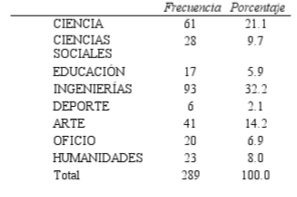
\includegraphics[scale=.63]{res1}
	\\Cuadro No. 1 : Frecuencia y porcentaje de las categor�as que 
	representan las carreras tentativas m�s populares.\\ 
		\bigskip
		\centering
		\justify 
		Luego de analizar todas y cada una de las respuestas que  los estudiantes ingresaron en la encuesta, se procede a clasificar las respuestas 	en 8 categor�as. De esta manera, se logra encontrar a que rama pertenecen las carreras tentativas que los estudiantes de la Universidad manifiestan como favoritas.\\
\end{itemize} 

	 
\begin{itemize}
	 \item Estudiantes que escogieron su carrera tentativa como universitaria:\\
	 \bigskip
	 \centering
	 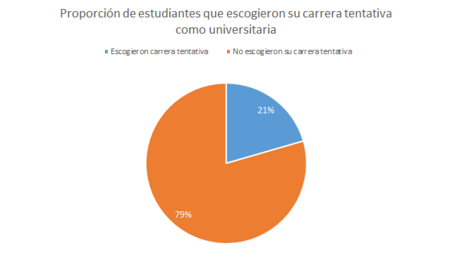
\includegraphics[scale=.73]{res2}
	 \\Gr�fica No. 1 : Porcentaje de estudiantes que escogieron su carrera
	 tentativa como universitaria.\\
	 \bigskip
	 \centering
	 \justify 
	 Por medio de una de las preguntas dicot�micas que tiene la encuesta
	 se logra hacer una proporci�n sobre los estudiantes que si logran escoger su carrera tentativa como universitaria, as� como los que no logran seguirla. \\
	  
\end{itemize}  
	  
